\chapter{Diplexer}
\label[appendix]{sec:annex_a}

Each diplexer unit of HIFI contains a Martin--Puplett interferometer~\parencite{martin1982polarizing}.
\Cref{fig:diplexer} illustrates its principle.

\begin{figure}[h]
    \centering
    \input{diplexer.pdf_tex}
    \caption{Schematic representation of a Martin--Puplett interferometer.}
    \label{fig:diplexer}
\end{figure}

\begin{enumerate}
    \item
    A wire-grid polarizer splits an input wave (purple) in two.
    \item
    The reflected (blue) and transmitted (red) waves follow two different paths
    \item
    The mirror
    The grid is oriented to satisfy three conditions:
    the reflected and transmitted waves must
    \begin{itemize}[nolistsep,noitemsep]
        \item propagate at right angle from each other,
        \item 
        \item carry the same power.
    \end{itemize}
    The first condition relates the plane of the grid to the direction of propagation of the wave: the angle of incidence must be~\SI{45}{\degree}.
    The second condition relates the orientation of the wires inside that plane to the polarization of the incoming wave: the 
\end{enumerate}
carries one half of the original power, and 

The rooftop mirrors are oriented so that the input waves are reflected back toward the grid with their polarization rotated by~\SI{90}{\degree} (see~\cref{fig:rooftop_polar}): if the first encounter with the grid is reflective then the second is transmissive and vice versa.

The two waves propagating toward the mixer can be seen as two components of a single output wave (principle of superposition).
On the figure, the dots on the paths of a wave represent the crests of that wave;
we can see that the blue and red dots are not in phase when they reach the mixer.
The phase difference is a function of the length of the mobile arm (red path on~\cref{fig:diplexer}) and the wave frequency.

The phase difference between the two components of the output wave determines the polarization of that output wave.
If the phase difference is~\SI{0}{\degree} or \SI{180}{\degree}, the output wave is linearly polarized; \SI{90}{\degree} and \SI{270}{\degree} give a circular polarization, and in all the other cases the polarization is elliptic.



\begin{figure}[b]
    \centering
    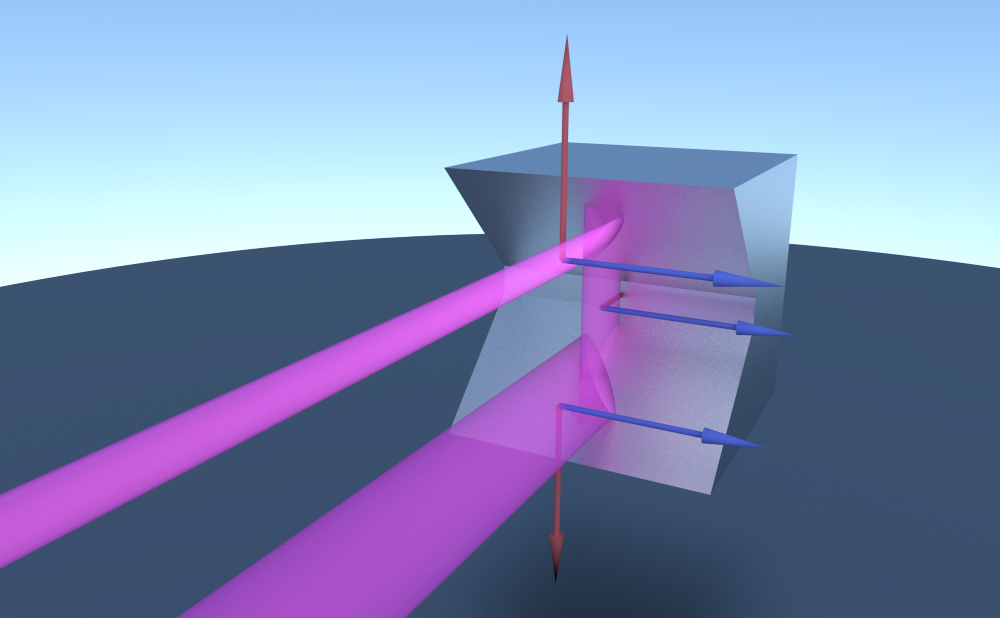
\includegraphics[width=\textwidth]{rooftop_polar_lowres}
    \caption{
        Rooftop mirrors flip the direction of one polarization and keep the other constant.
        What is shown in purple is not the beam: the beam (not represented)
        has a circular cross-section and shines on both planes of the rooftop mirror equally and simultaneously.
        Instead, the purple path represents both the direction of propagation and the plane of polarization of a particular beam.
        The blue and red arrows follow a reference frame attached to a beam before (top), during (middle), and after (bottom) reflection, shown in a global reference frame.
        Upon reflection, but blue direction is not modified but the red direction has flipped.
        Consequently, if a beam is linearly polarized at~\SI{+45}{\degree} in the global
        frame (which is the case illustrated by the purple path),
        then its reflection is polarized at~\SI{-45}{\degree} in the same global frame.
        In effect, the rooftop mirror has rotated the polarization of that beam by
        \SI{90}{\degree}.
        If the beam had been polarized along the red or blue axis, the rooftop mirror would have had no effect on the polarization plane of the beam.
    }
    \label{fig:rooftop_polar}
\end{figure}

\begin{figure}[b]
    \centering
    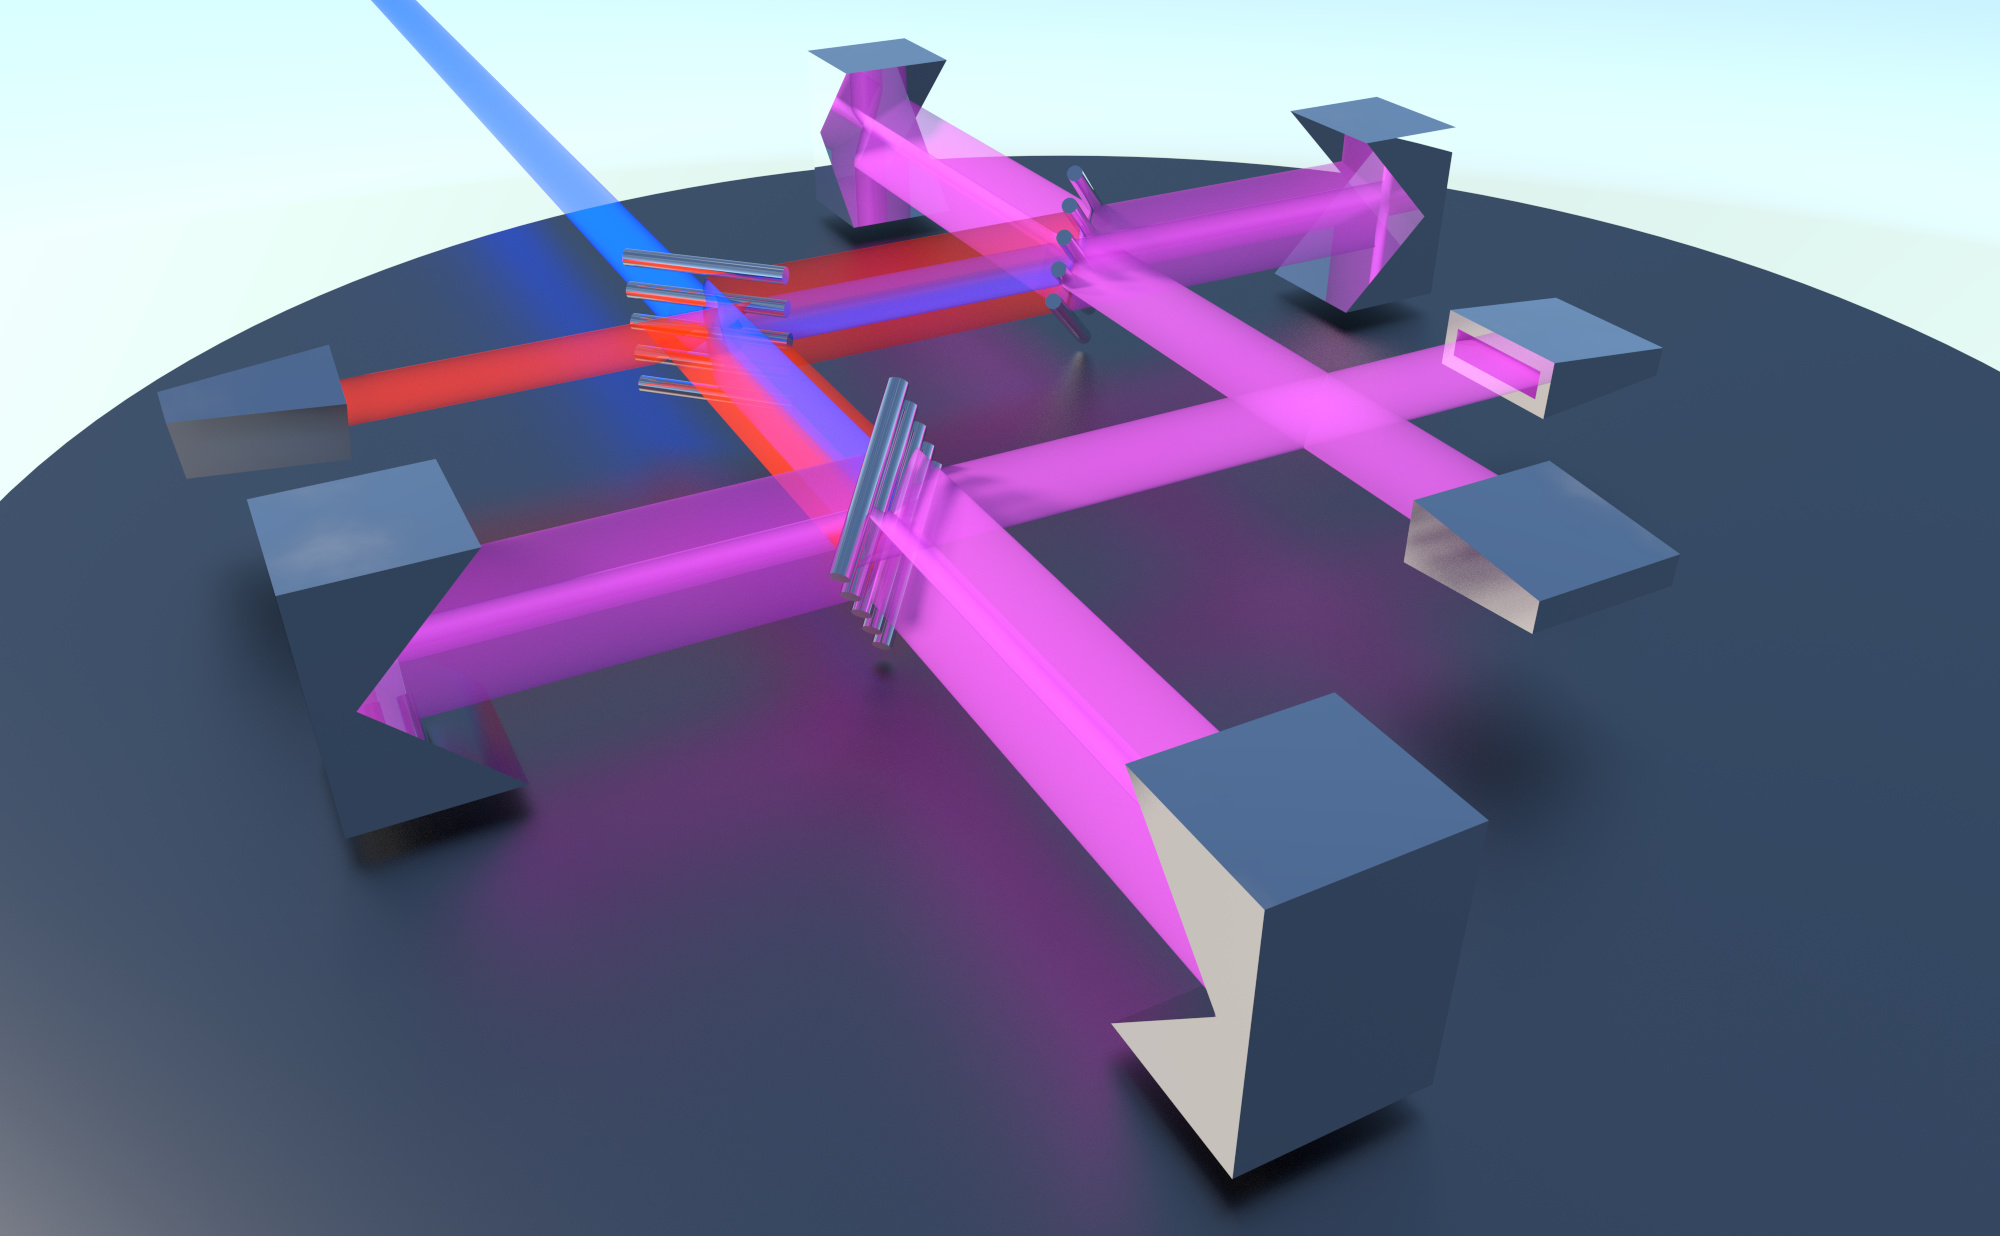
\includegraphics[width=\textwidth]{diplexer_render_lowres}
    \caption{
        Schematic 3D representation of the diplexer units in HIFI.
        The blue beam represents the signal from the sky, the red beam is the LO signal,
        and the purple beams are a superposition of the two.
        \emph{First}, the LO and sky signal are split in two by a wire-grid polarizer.
        The polarization of the beams is represented by their tilt.
        \emph{Second}, the LO and sky beams have their polarizations lined-up by the diplexers.
        Each diplexer is made of one wire-grid polarizer and two rooftop mirrors.
        \emph{Finally}, the combined beams of the LO and the sky enter the horns to be mixed.
    }
    \label{fig:diplexer_render_appendix}
\end{figure}



An ideal diplexer is modeled by
\begin{align}
    G_\text{sky}(f)
    &=
    \cos
    \left(
        2 \pi
        \frac{df}{c}
    \right)^2
    \\
    G_\text{LO}(f)
    &=
    1 - G_\text{sky}(f)
    \label{eq:diplexer_coupling_model}
\end{align}
with $G_\text{sky}$ and $G_\text{LO}$ the coupling of the mixer to the sky and the LO,
$f$ the wave frequency,
$d$ the length difference between the two arms of the interferometer,
and $c$ the speed of light in the propagation medium (vacuum in our case).

This frequency-dependence implies that the coupling of the mixer to the LO and the sky cannot be optimal over a wide range of frequencies.
In HIFI, the nominal pathlength difference is chosen so that the mixer is maximally coupled to the LO at the LO frequency~$f_\text{LO}$,
and to the sky at $f_\text{LO} \pm \SI{6}{\giga\hertz}$.
This value of~\SI{6}{\giga\hertz} corresponds to the center of the bandwidth of the mixer, which ranges from \num{4} to \SI{8}{\giga\hertz}.
As a result, the coupling of the mixer to the sky is optimal at the center of the spectrum.
This is illustrated by the diplexer coupling model on the top plot of~\cref{fig:diplexer_ideal}.
In that ideal case, the sideband ratio SBR defined as
\begin{equation}
    \text{SBR} =
    \frac{
        G_\text{USB}
    }{
        G_\text{LSB} + G_\text{USB}
    }
\end{equation}
is constant over the whole bandwidth and equals \num{0.5}, which means that the mixer couples to both sidebands equally, as shown on the bottom plot of~\cref{fig:diplexer_ideal}.

At the edges of the sidebands, the coupling to the sky is lower and the coupling to the LO is higher.
Since the LO is a source of thermal noise, the signal-to-noise ratio decreases toward the edges of the spectrum.
This can be seen on the baseline of~\cref{fig:co98_full_bandwidth}.

\begin{figure}
    \centering
    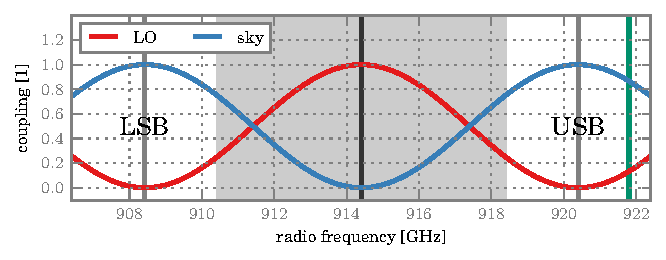
\includegraphics{diplexer_coupling_ideal}
    \caption*{
        Coupling of the mixer to the LO and the sky for an optimally-tuned diplexer.
        The mixer--LO coupling is maximal at the LO frequency
        (black vertical line at~\SI{914.4045}{\giga\hertz}).
        The mixer--sky coupling is maximal at the center of the lower and upper sidebands (gray vertical lines LSB and USB).
    }
    \bigskip
    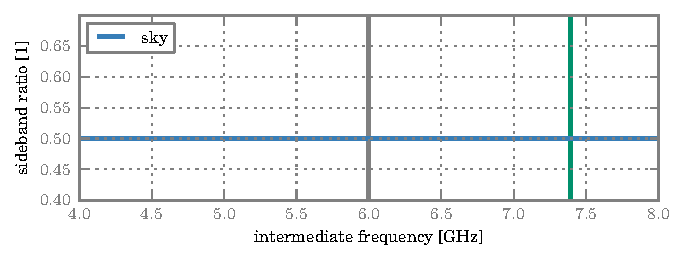
\includegraphics{diplexer_sbr_ideal}
    \caption*{
        Sideband ratio of the mixer--sky coupling for an optimally-tuned diplexer.
        The constant sideband ratio of \num{0.5} indicates that the LSB and the USB contribute in equal measure to each channel of the spectrum.
    }
    \caption{
        Model of the coupling and the sideband ratio for an optimally-tuned diplexer.
        The green vertical lines show the rest frequency of the \transition{CO}{8}{7} transition.
        The LO frequency is~\SI{914.4045}{\giga\hertz}.
        The difference in length of the two arms of the diplexer is~\SI{12.5405}{\milli\meter}.
    }
    \label{fig:diplexer_ideal}
\end{figure}

Because each LO frequency requires its own optical pathlength difference, 
one of the rooftop mirrors can be translated.
This translation is commanded by an electric current applied to an actuator.
The equation relating~$I$, diplexer actuator current in milliampere, to~$d$, interferometer arm length difference in millimeter, is
\begin{equation}
    d = d_0 + 27.5 \frac{2\pi}{360}(a I^2 + b I)\text{.}
\end{equation}
The currents $I$ are given in~\cref{tab:los_and_dacs}.
The remaining parameters $d_0$, $a$ and $b$ are given in~\cref{tab:diplexer_params}.
These parameters are very well known and have remained constant (sub-micrometer precision) during the entire mission \parencite{mueller2014flight}.

\begin{table}
    \centering
    \begin{tabular}{cccc}
        \toprule
        mixer &
        $a$ [\si{\degree\per\milli\ampere\squared}]
        &
        $b$ [\si{\degree\per\milli\ampere}]
        &
        $d_0$ [\si{\milli\meter}]
        \\
        \midrule
        3h    &  \num{-0.003991} & 0.1976 & 12.3354\\
        3v    &  \num{-0.004821} & 0.2155 & 12.1231\\
        4h    &  \num{-0.004348} & 0.1722 & 12.3490\\
        4v    &  \num{-0.003553} & 0.1791 & 12.5395\\
        6h    &  \num{-0.002401} & 0.1735 & 21.0532\\
        6v    &  \num{-0.005408} & 0.2100 & 20.8718\\
        7h    &  \num{-0.002272} & 0.1661 & 20.7954\\
        7v    &  \num{-0.002757} & 0.1586 & 20.7666\\
        \bottomrule
    \end{tabular}
    \caption{Parameters used to convert diplexer actuator currents to interferometer arm length difference.
    We use the mixers 3h and 4h in our study.}
    \label{tab:diplexer_params}
\end{table}
